
\chapter*{Animating the Wave Equation: Staggered Leapfrog}
\addcontentsline{toc}{chapter}{Animating the Wave Equation: Staggered Leapfrog} 
In the last couple of labs we handled the wave equation by Fourier analysis,
turning the partial differential equation into a set of ordinary differential equations using separation of variables.1 But separating the variables and expanding
in orthogonal functions is not the only way to solve partial differential equations,
and in fact in many situations this technique is awkward, ineffective, or both. In
this lab we will study another way of solving partial differential equations using a
spatial grid and stepping forward in time. As an added attraction, this method
automatically supplies a beautiful animation of the solution. There are several
algorithms of this type that can be used on wave equations, so this is just an
introduction to a larger subject. The method we will show you here is called
staggered leapfrog; it is the simplest good method that we know


\section*{The wave equation with staggered leapfrog}
\addcontentsline{toc}{section}{The wave equation with staggered leapfrog} 
Consider again the classical wave equation with wave speed c.

\begin{equation}\label{eq:51}
	\frac{\partial^2 y}{\partial t^2} - c^2 \frac{\partial^2 y}{\partial x^2} = 0
\end{equation}
For a string, the wave speed is related to tension and density via $c = \sqrt{T / \mu} $ The
boundary conditions are usually either of Dirichlet type (values specified):
\begin{equation}\label{eq:52}
	y(0,t) = f_{left}(t) ; y(L,t) = f_{right}(t)
\end{equation}
or of Neumann type (derivatives specified):
\begin{equation}\label{eq:53}
	\frac{\partial y}{\partial x} (0)  = g_{left}(t) ; \frac{\partial y}{\partial x} (L)  = g_{right}(t)
\end{equation}
Sometimes mixed boundary conditions specify a relation between the value
and derivative, as at the bottom of the hanging chain. In any case, some set of
conditions at the endpoints are required to solve the wave equation. It is also
necessary to specify the initial state of the string, giving its starting position and
velocity as a function of position:
\begin{equation}\label{eq:54}
	y(x,t = 0) = y_0(x) \quad ; \quad \frac{\partial y(x,t)}{\partial t} \vert_{t=0} = v_0 (x)
\end{equation}
Both of these initial conditions are necessary because the wave equation is second
order in time, just like Newton\rq s second law, so initial displacement and velocity
must be specified at each point to find a unique solution.
To numerically solve the classical wave equation via staggered leapfrog we
approximate both the temporal and spatial derivatives in Eq.\ref{eq:51} with centered
finite differences, like this:
\begin{equation}\label{eq:55}
\begin{aligned}
&\frac{\partial^{2} y}{\partial t^{2}} \approx \frac{y_{j}^{n+1}-2 y_{j}^{n}+y_{j}^{n-1}}{\tau^{2}} \\
&\frac{\partial^{2} y}{\partial x^{2}} \approx \frac{y_{j+1}^{n}-2 y_{j}^{n}+y_{j-1}^{n}}{h^{2}}
\end{aligned}
\end{equation}
In this notation, spatial position is indicated by a subscript $j$, referring to grid
points $x_j$, while position in time is indicated by superscripts $n$, referring to time
points $t_n$ so that $y(x_j,t_n) = y_j^n$. The time steps and the grid spacings are assumed to be uniform with time step called
$\tau$ and grid spacing called $h$. The staggered leapfrog algorithm aims to find $y_j$ one time step into the future, denoted by $y_j^{n+1}$,
from the current and previous values of $y_j$. To derive the algorithm put Eqs.\ref{eq:55} into Eq. \ref{eq:51} and solve for $y_j^{n+1}$ to find
\begin{equation}\label{eq:56}
	y_j^{n+1} = 2y_j^n - y_j^{n-1} + \frac{c^2 \tau^2}{h^2}(y_{j+1}^n - 2y^n_j + y^n_{j-1})
\end{equation}

\begin{problem}\label{P5.1} Derive Eq. \ref{eq:56} using the approximate second derivative formulas. This is
really simple, so just do it on paper.\end{problem}
Equation \ref{eq:56} can only be used at interior spatial grid points because the
$ j + 1 {or} j-1$  indices reach beyond the grid at the first and last grid points. The
behavior of the solution at these two end points is determined by the boundary
conditions. Since we will want to use both fixed value and derivative boundary
conditions, let\rq s use a cell-centered grid with ghost points (with $N$ cells and $N+2$ grid points) so we can easily handle both types without changing our grid. If the values at the ends are specified we have 
\begin{equation}\label{eq:57}
\begin{gathered}
\frac{y_{0}^{n+1}+y_{1}^{n+1}}{2}=f_{\text {left }}\left(t_{n+1}\right) \Rightarrow y_{0}^{n+1}=-y_{1}^{n+1}+2 f_{\text {left }}\left(t_{n+1}\right) \\
\frac{y_{N+1}^{n+1}+y_{N}^{n+1}}{2}=f_{\text {right }}\left(t_{n+1}\right) \Rightarrow y_{N+1}^{n+1}=-y_{N}^{n+1}+2 f_{\text {right }}\left(t_{n+1}\right)
\end{gathered}
\end{equation}
If the derivatives are specified then we have
\begin{equation}\label{eq:58}
\begin{aligned}
&\frac{y_{1}^{n+1}-y_{0}^{n+1}}{h}=g_{\text {left }}\left(t_{n+1}\right) \Rightarrow y_{0}^{n+1}=y_{1}^{n+1}-h g_{\text {left }}\left(t_{n+1}\right) \\
&\frac{y_{N+1}^{n+1}-y_{N}^{n+1}}{h}=g_{\text {right }}\left(t_{n+1}\right) \Rightarrow y_{N+1}^{n+1}=y_{N}^{n+1}+h g_{\text {right }}\left(t_{n+1}\right)
\end{aligned}
\end{equation}
To use staggered leapfrog, we first advance the solution at all interior points to
the next time step using Eq. \ref{eq:56}, then we apply the boundary conditions using
the appropriate equation from Eqs. \ref{eq:57}-\ref{eq:58} to find the values of y at the end
points, and then we are ready to take another time step.
The staggered leapfrog algorithm in Eq. \ref{eq:56} requires not just y at the current
time level $ y_j^n$ but also $y$ at the previous time level $y^{n−1}_j$. This means that we\rq ll need
to keep track of three arrays: an array y for the current values $ y_j^n$, an array yold
for the values at the previous time step $ y_j^{n-1}$, and an array ynew for the values
at the next time step $ y_j^{n+1}$. At time $t = 0$ when the calculation starts, the initial
position condition gives us the current values $ y_j^n$ , but we\rq ll have to make creative
use of the initial velocity condition to create an appropriate yold to get started.
To see how this works, let\rq s denote the initial values of y on the grid by $ y_j^0 $, the
values after the first time step by $ y_j^{1} $, and the unknown previous values (yold) by
$ y_j^{-1} $. A centered time derivative at $t = 0$ turns the initial velocity condition from
Eq. \ref{eq:54} into
\begin{equation}\label{eq:59}
\frac{y_j^1 - y_j^{-1}}{2 \tau} = v_0(x_j)
\end{equation}
This gives us an equation for the previous values $y_j^{-1}$ , but it is in terms of the
still unknown future values $y_j^{1}$. However, we can use Eq. \ref{eq:56} to obtain another
relation between $y_j^{1}$and $y_j^{-1}$. Leapfrog at the first step ($n = 0$) says that
\begin{equation}\label{eq:510}
y_j^1 = 2Y^0_j - y_j^{-1} + \frac{c^2 \tau^2}{h^2}(y^0_{j+1}-2y^0_j+y^0_{j-1})
\end{equation}
If we insert this expression for $y^1_j$ into Eq. \ref{eq:59}, we can solve for $y^{-1}_j $ in terms of
known quantities:
\begin{equation}\label{eq:511}
y_j^{-1} = Y^0_j - v_0(x_j)\tau + \frac{c^2 \tau^2}{2h^2}(y^0_{j+1}-2y^0_j+y^0_{j-1})
\end{equation}

\begin{problem}\label{P5.2} Derive Eq. \ref{eq:511} from Eqs. \ref{eq:59} and \ref{eq:510}. Again, just use paper and pencil.
OK; we are now ready to code the staggered leapfrog algorithm.\end{problem}
\begin{problem}\label{P5.3} 

\begin{enumerate}[label=(\alph*)]
\item Start by making a cell-centered $x$ grid with ghost points over the region
$0 \leq x \leq L$, with $L = 1$ m. Use $N = 200$ cells, so you have 202 grid
points. Define the initial displacement $y$ as Gaussian bump with 1 cm
amplitude in the middle of the string, like this
\begin{lstlisting}
y = 0.01 * np.exp(-(x-L/2)**2 / 0.02)
\end{lstlisting}
and the initial velocity $vy$ to be zero everywhere along the string. Used
fixed-value boundary conditions, with $y(0) = 0$ and $y(L) = 0$. Plot the
initial position just to make sure your grid is right and that your initial
position array looks reasonable
\item Assume that the wave speed on this string is $c = 2$ m/s, and pick
the time step as $tau = 0.2*h/c$. (We\rq ll explore this choice more
later.) Then create a variable yold using Eq. \ref{eq:511}, and enforce the boundary conditions on yold. As you write this code, don\rq t write a
bunch of for loops to iterate through all the points. Instead, assign all
interior points at once using the NumPy array colon indexing method
(e.g. $y[1:-1]$ accesses all the interior points of $y$) and then set the
boundary conditions explicitly
\item Now it is time to code the main staggered leapfrog algorithm and make
an animation of the solution. Since it has been a couple of labs since
we made an animation, here is a framework for the code to remind
you of the basic animation commands:
	\marginpar{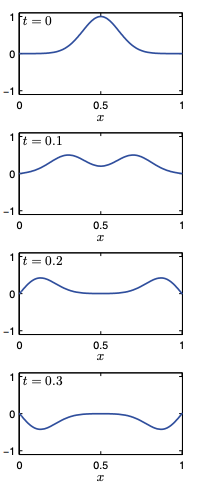
\includegraphics[width=\marginparwidth]{fig51}\captionof{figure}{Snapshots of the evolution of a wave on a string with fixed ends and an initial displacement but no initial velocity. (See Problem \ref{P5.3}(b))}\label{fig:25}}
\begin{lstlisting}
ynew = np.zeros_like(y)
j = 0
t = 0
tmax = 2
plt.figure(1) # Open the figure window
# the loop that steps the solution along
while t < tmax:
j = j+1
t = t + tau
# Use leapfrog and the boundary conditions
# to load ynew with y at the next time
# step using y and yold
# update yold and y for next timestep
# remember to use np.copy
# make plots every 50 time steps
if j % 50 == 0:
plt.clf() # clear the figure window
plt.plot(x,y,'b-')
plt.xlabel('x')
plt.ylabel('y')
plt.title('time={:1.3f}'.format(t))
plt.ylim([-0.03,0.03])
plt.xlim([0,1])
plt.draw() # Draw the plot
plt.pause(0.1) # Give the computer time to draw
\end{lstlisting}
The actual staggered leapfrog code is missing above. You’ll need to
write that. Run the animations long enough that you can see the
reflection from the ends and the way the two pulses add together and
pass right through each other.
\item Once you have it running, experiment with various time steps $\tau$. Show
by numerical experimentation that if$ \tau > h/c$ the algorithm blows up
spectacularly. This failure is called a numerical instability and we
will be trying to avoid it all semester. This limit is called the CourantFriedrichs-Lewy condition, or sometimes the CFL condition, or 

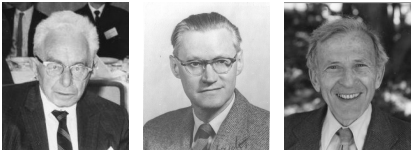
\includegraphics[width=\marginparwidth]{fig52}\captionof{figure}{Richard Courant (left), Kurt Friedrichs (center), and Hans Lewy (right) described the CFL instability condition in 1928 .}\label{fig:26}


sometimes (unfairly) just the Courant condition
\item Change the boundary conditions so that $ \frac{\partial y}{\partial x} = 0 $ at each end and watch
how the reflection occurs in this case.
\item Change the initial conditions from initial displacement with zero
velocity to initial velocity with zero displacement. Use an initial Gaussian velocity pulse just like the displacement pulse you used earlier
and use fixed-end boundary conditions. Watch how the wave motion
develops in this case. (You will need to change the y-limits in the axis
command to see the vibrations with these parameters.) Then find a
slinky, stretch it out, and whack it in the middle to verify that the math
does the physics right.

\end{enumerate}
\end{problem}
\section*{The damped wave equation}

\addcontentsline{toc}{section}{The damped wave equation} 
We can modify the wave equation to include damping of the waves using a linear
damping term, like this:
\begin{equation}\label{eq:512}
	\frac{\partial^2 y}{\partial t^2} + \Upsilon \frac{\partial y}{\partial t} - c^2 \frac{\partial^2 y}{\partial x^2} = 0
\end{equation}
\marginpar{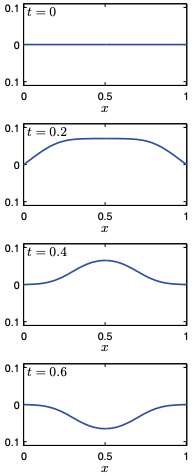
\includegraphics[width=\marginparwidth]{fig53}\captionof{figure}{ Snapshots of the evolution of a wave on a string with fixed ends and no initial displacement but with an initial velocity. (See Problem \ref{P5.3}(f))}\label{fig:27}}
with $c$ constant. The staggered leapfrog method can be used to solve Eq. \ref{eq:512}
also. To do this, we use the approximate first derivative formula
\begin{equation}\label{eq:513}
\frac{\partial y}{\partial t } \approx = \frac{y_j^{n+1} - y_j^{n-1}}{2 \tau}
\end{equation}
along with the second derivative formulas in Eqs. \ref{eq:55} and find an expression for
the values one step in the future:
\begin{equation}\label{eq:514}
y^{n+1}_j = \frac{1}{2+ \Upsilon \tau}(4y^n_j-2y^{n-1}_j+ \Upsilon \tau y^{n-1}_j + \frac{2c^2 \tau^2}{h^2}(y^n_{j+1} - 2y^n_j + y^n_{j-1}))
\end{equation}
\begin{problem}\label{P5.4} 
\begin{enumerate}[label=(\alph*)]
	\item Derive Eq. \ref{eq:514}.
	\item Find a new formula for the initial value of yold using Eqs.\ref{eq:59} and
\ref{eq:514}. When you get the answer, ask your TA or instructor to check to
see if you got it right.
\item Modify your staggered leapfrog code to include damping with $ \Upsilon = 0.2$.
Then run your animation with the initial conditions in Problem \ref{P5.3}(c)
and verify that the waves damp away. You will need to run for about
25 s and you will want to use a big skip factor so that you don\rq t have
to wait forever for the run to finish. Include some code to record the
maximum value of $y(x)$ over the entire grid as a function of time and
then plot it as a function of time at the end of the run so that you can
see the decay caused by $\Upsilon$. The decay of a simple harmonic oscillator
is exponential, with amplitude proportional to $e^{−\Upsilon^{ t/2}}$. Scale this time
decay function properly and lay it over your maximum y plot to see if
it fits. Can you explain why the fit is as good as it is? (Hint: think about
doing this problem via separation of variables.)

\end{enumerate}
\end{problem}
	\marginpar{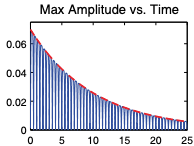
\includegraphics[width=\marginparwidth]{fig54}\captionof{figure}{The maximum amplitude of oscillation decays exponentially for the damped wave equation. (Problem \ref{P5.4} (c))}\label{fig:28}}
\section*{The damped and driven wave equation}
\addcontentsline{toc}{section}{The damped and driven wave equation} 
Finally, let\rq s look at what happens when we add an oscillating driving force to our
string, so that the wave equation becomes
\begin{equation}\label{eq:515}
\frac{\partial^2 y}{\partial t^2} + \Upsilon \frac{\partial y}{\partial t}-c^2\frac{\partial^2 y}{\partial x^2} = \frac{f(x)}{\mu} \cos(\omega t )
\end{equation}

At the beginning of Lab 3 we discussed the qualitative behavior of this system.
Recall that if we have a string initially at rest and then we start to push and pull on
a string with an oscillating force/length of $f(x)$, we launch waves down the string.
These waves reflect back and forth on the string as the driving force continues
to launch more waves. The string motion is messy at first, but the damping in
the system causes the the transient waves from the initial launch and subsequent
reflections to eventually die away. In the end, we are left with a steady-state
oscillation of the string at the driving frequency $\omega$.
Now that we have the computational tools to model the time evolution of the
system, let\rq s watch this behavior.
\begin{problem}\label{P5.5} 

\begin{enumerate}[label=(\alph*)]
\item Re-derive the staggered leapfrog algorithm to include both driving
and damping forces as in Eq. \ref{eq:515}.
\item Modify your code from Problem \ref{P5.4} to use this new algorithm. We\rq ll
have the string start from rest, so you don\rq t need to worry about finding
yold. Just set $y = 0$ and $yold = 0$ and enter the time-stepping loop.
This problem involves the physics of waves on a real guitar string,
so we\rq ll need to use realistic values for our parameters. Use $T = 127$,
$ \mu = 0.003$, and$ L = 1.2$ (in SI units) and remember that $ c = \sqrt{T / \mu}$. Use the same driving force as in Problem \ref{P3.2}(a)

\begin{equation}\label{eq:516}
f(x)= \begin{cases}0.73 & \text { if } 0.8 \leq x \leq 1 \\ 0 & \text { otherwise }\end{cases}
\end{equation}
and set the driving frequency at $\omega = 400$. Choose a damping constant
$\Upsilon$ that is the proper size to make the system settle down to steady state
after 20 or 30 bounces of the string. (You will have to think about the
value of  $\omega$ that you are using and about your damping rate result from
problem \ref{P5.4} to decide which value of $\Upsilon$ to use to make this happen.)
Run the model long enough that you can see the transients die away
and the string settle into the steady oscillation at the driving frequency.
You may find yourself looking at a flat-line plot with no oscillation at
all. If this happens look at the vertical scale of your plot and remember
that we are doing real physics here. If your vertical scale goes from −1
to 1, you are expecting an oscillation amplitude of 1 meter on your
guitar string. Compare the steady state mode to the shape found in
Problem \ref{P3.2}(a) (see Fig. \ref{fig:31}).
Then run again with $ \omega = 1080 $, which is close to a resonance, and again
see the system come into steady oscillation at the driving frequency.
\end{enumerate}
\end{problem}
	\marginpar{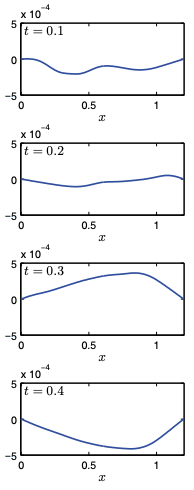
\includegraphics[width=\marginparwidth]{fig55}\captionof{figure}{Snapshots of the evolution a driven and damped wave with $\omega=400$. As the transient behavior dies out, the oscillation goes to the resonant mode. To make the pictures more interesting, the string was not started from rest in these plots. (In Problem \ref{P5.5} you start from rest for easier coding.]}\label{fig:29}}
